
%==============================================================%

本書は初めて領域気象気候モデル {\scalerm}
を利用する人に向けた解説書である。
気象気候ライブラリー{\scalelib}  version \version に対応した説明を記載する。
\scalelib の現バージョンには、領域モデル\scalerm と全球モデル\scalegm が含まれる。
本版では、\scalerm の使い方についてのみ詳しく述べる。
\scalegm については、次版で詳しく記載される予定である。
%\scalerm の使い方を通して、\scalelib を他のモデルからの呼び出す方法を
%習得することも可能です。

本書の構成は次の通りです。
第\ref{part:overview}部では SCALE の概要、
第\ref{part:install}部では必要な環境とインストール方法について説明する。
続いて、第\ref{chap:tutorial_ideal}章では理想実験、第\ref{chap:tutorial_real}章では現実大気実験を例にして、\scalerm の基本的な操作方法を説明する。
これらの章はひと繋がりのチュートリアルとなっており、
\scalerm を初めて使うユーザは一通り通読することを推奨する。
第\ref{part:basic_usel}部と第\ref{part:advance_use}部では、
モデルの設定の変更方法を記載し、また利用できるデータ形式やツールを説明する。
これらの各章は基本的にその中で閉じているので、辞書として用いることができる。

%%%
本書中の不明点やお気づきの点がございましたら、SCALE user's メーリングリスト\\
 \verb|scale-users@ml.riken.jp|までご連絡ください。



\section{\scalelib とは?} \label{subsec:scale_feature}
%--------------------------------------------------------------%

{\scalelib} (Scalable Computing for Advanced Library and Environment)は、
気候研究や天気予報を容易に様々な計算機上で行うためのソフトウェア・ライブラリである。
本ライブラリは、前処理からシミュレーション、後処理、解析に至るまで全ての過程を網羅し、
下記に挙げる長所を持つ。
\begin{itemize}
\item \scalelib は、「BSD-2ライセンス」のもとオープンソースソフトウェア
として提供している。
商用、非商用に関わらず自由な利用、改変、再配布が可能である。
\item \scalelib には、{\scalerm} (SCALE-Regional Model)
%SCALE-GM(SCALE-Global Model)
という領域モデルが含まれる。
\item \scalelib には、次節で説明するように様々なスキームが用意されている。
ユーザーが行いたい実験に合わせて適宜選択できる。
\item \scalelib では、\scalerm だけでなく他の数値モデルでも呼び出せる
物理過程のフレームワークを提供している。
\end{itemize}

ライセンスの詳細は、トップディレクトリ直下の\texttt{scale-\version/LICENSE}のファイルに記述されている。
\scalelib の使用前に一読されたい。
また、\scalelib のWebページ(\scaleweb)にもソフトウェアの説明が記載されているので必要に応じて参照されたい。

本節では、\scalelib の思想や実際のモデルとの関係について説明する。
\scalerm の実行とは直接的には関係しないため、必要なければ読み飛ばしても構わない。

\Item{\scalelib のライブラリとモデルの関係について}

\begin{figure}[htb]
\begin{center}
  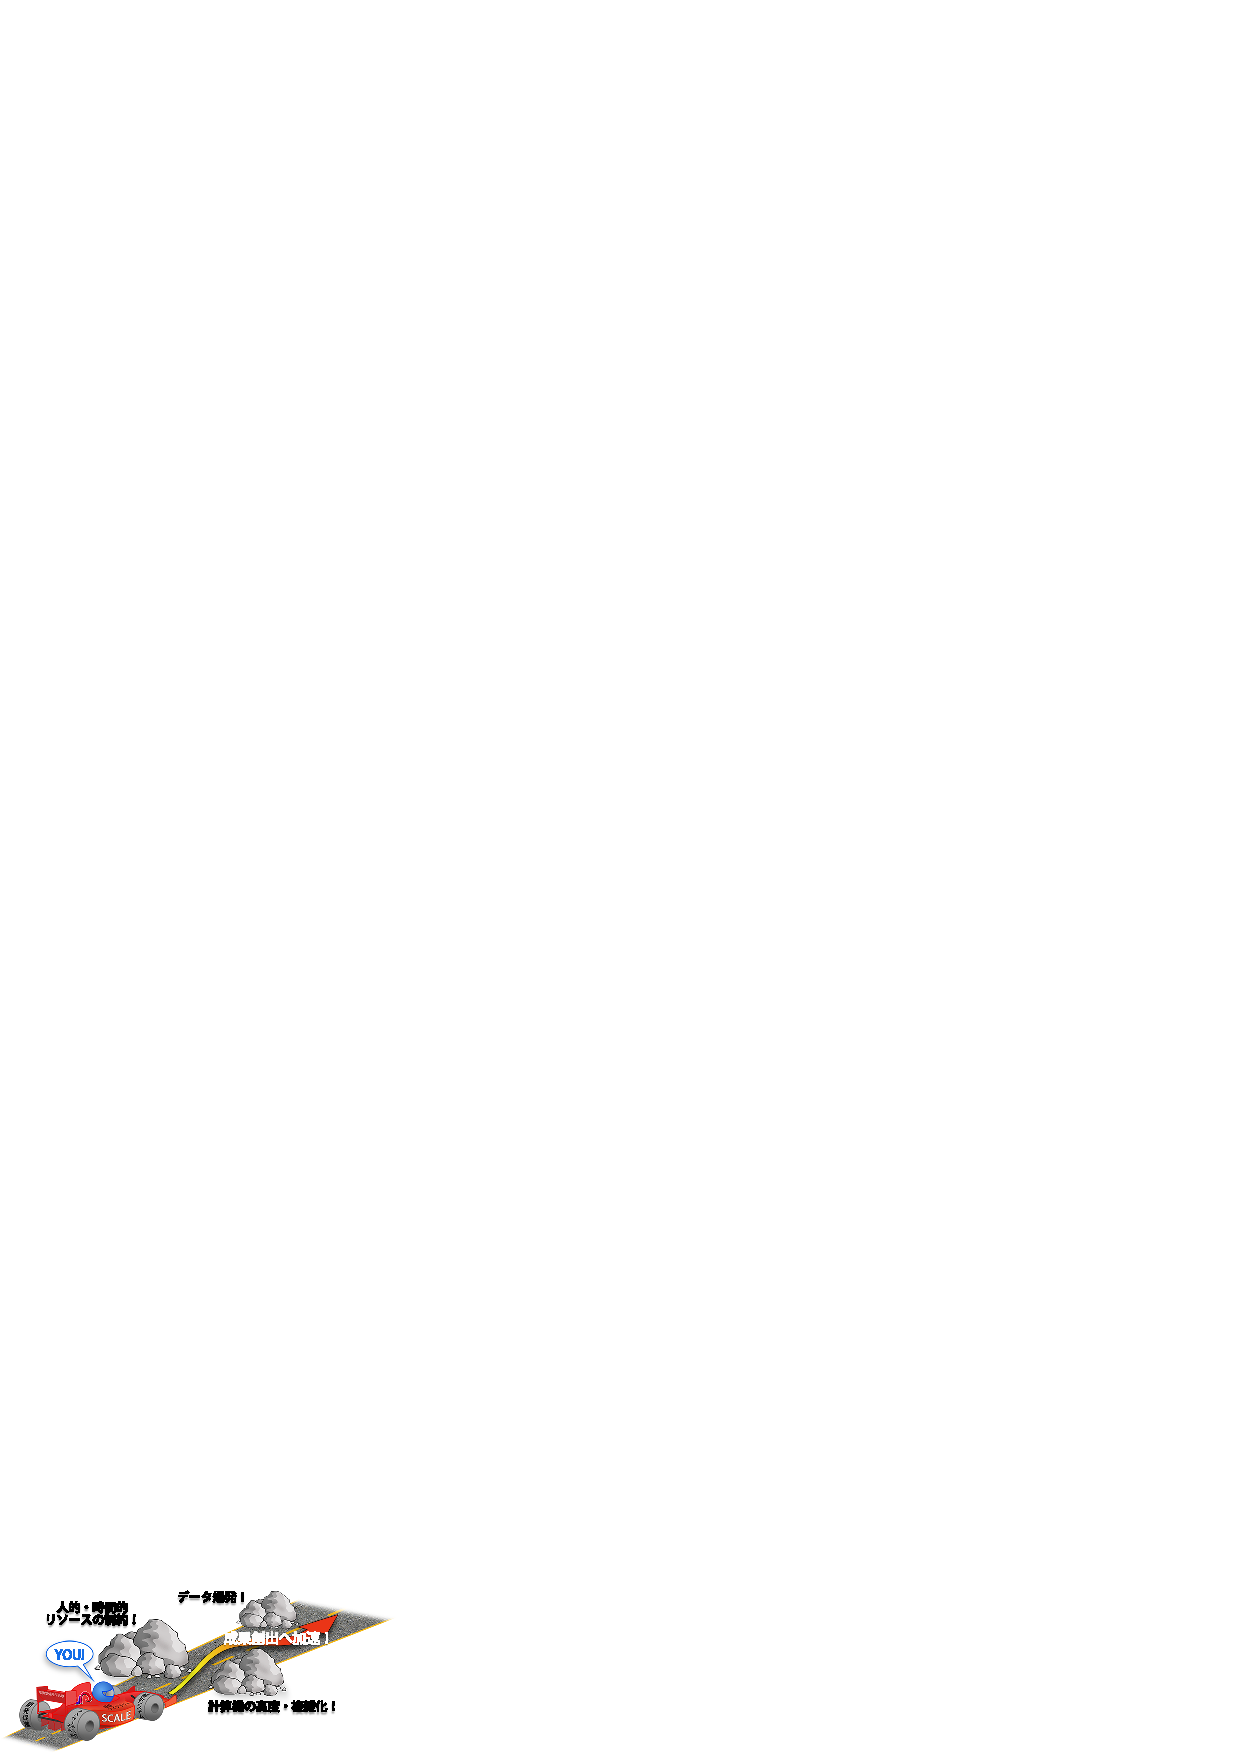
\includegraphics[width=0.9\hsize]{./../../figure/library.pdf}\\
  \caption{\scalelib のねらい}
  \label{fig:scale}
\end{center}
\end{figure}

\scalelib は幾つかの外部共同研究者と共に理化学研究所(RIKEN)で開発され、
その改良と拡張が継続的に行われている。
図 \ref{fig:scale}に\scalelib の思想の概念図を示す。
この図に示されるように、\scalelib は様々な問題に対応することを目指している。
\scalelib は、小型PCクラスターから次世代のスーパーコンピュータに至るまで様々な計算環境で広く用いられる事を念頭に開発されている。
この目的のため、気候・気象科学を専門とする科学者と計算機科学を専門とする科学者が
共同で開発している。

\scalerm は \scalelib ライブラリを大いに利用した数値モデルの一つであり、
図\ref{fig:scale-rm}に示すように \scalelib のパッケージに含まれる。
\scalelib は、並列プロセスの管理、ファイルの入出力、プロセス間の通信、格子情報の設定を行う。
また、\scalelib は、大気の流れのソルバ(力学コア)や雲微物理や大気放射等の物理過程も提供する。
その一方で、\scalerm は\scalelib が提供する機能を組み合わせることで構築されている。
\scalerm 自体は、大気の状態の入力データを予報変数として読み込んで保持し、
\scalelib の各コンポーネントを適宜呼び出すことで時間発展を計算する。
ユーザは行いたい実験に応じて、各コンポーネントのスキームを選択できる。

\begin{figure}[hbt]
\begin{center}
  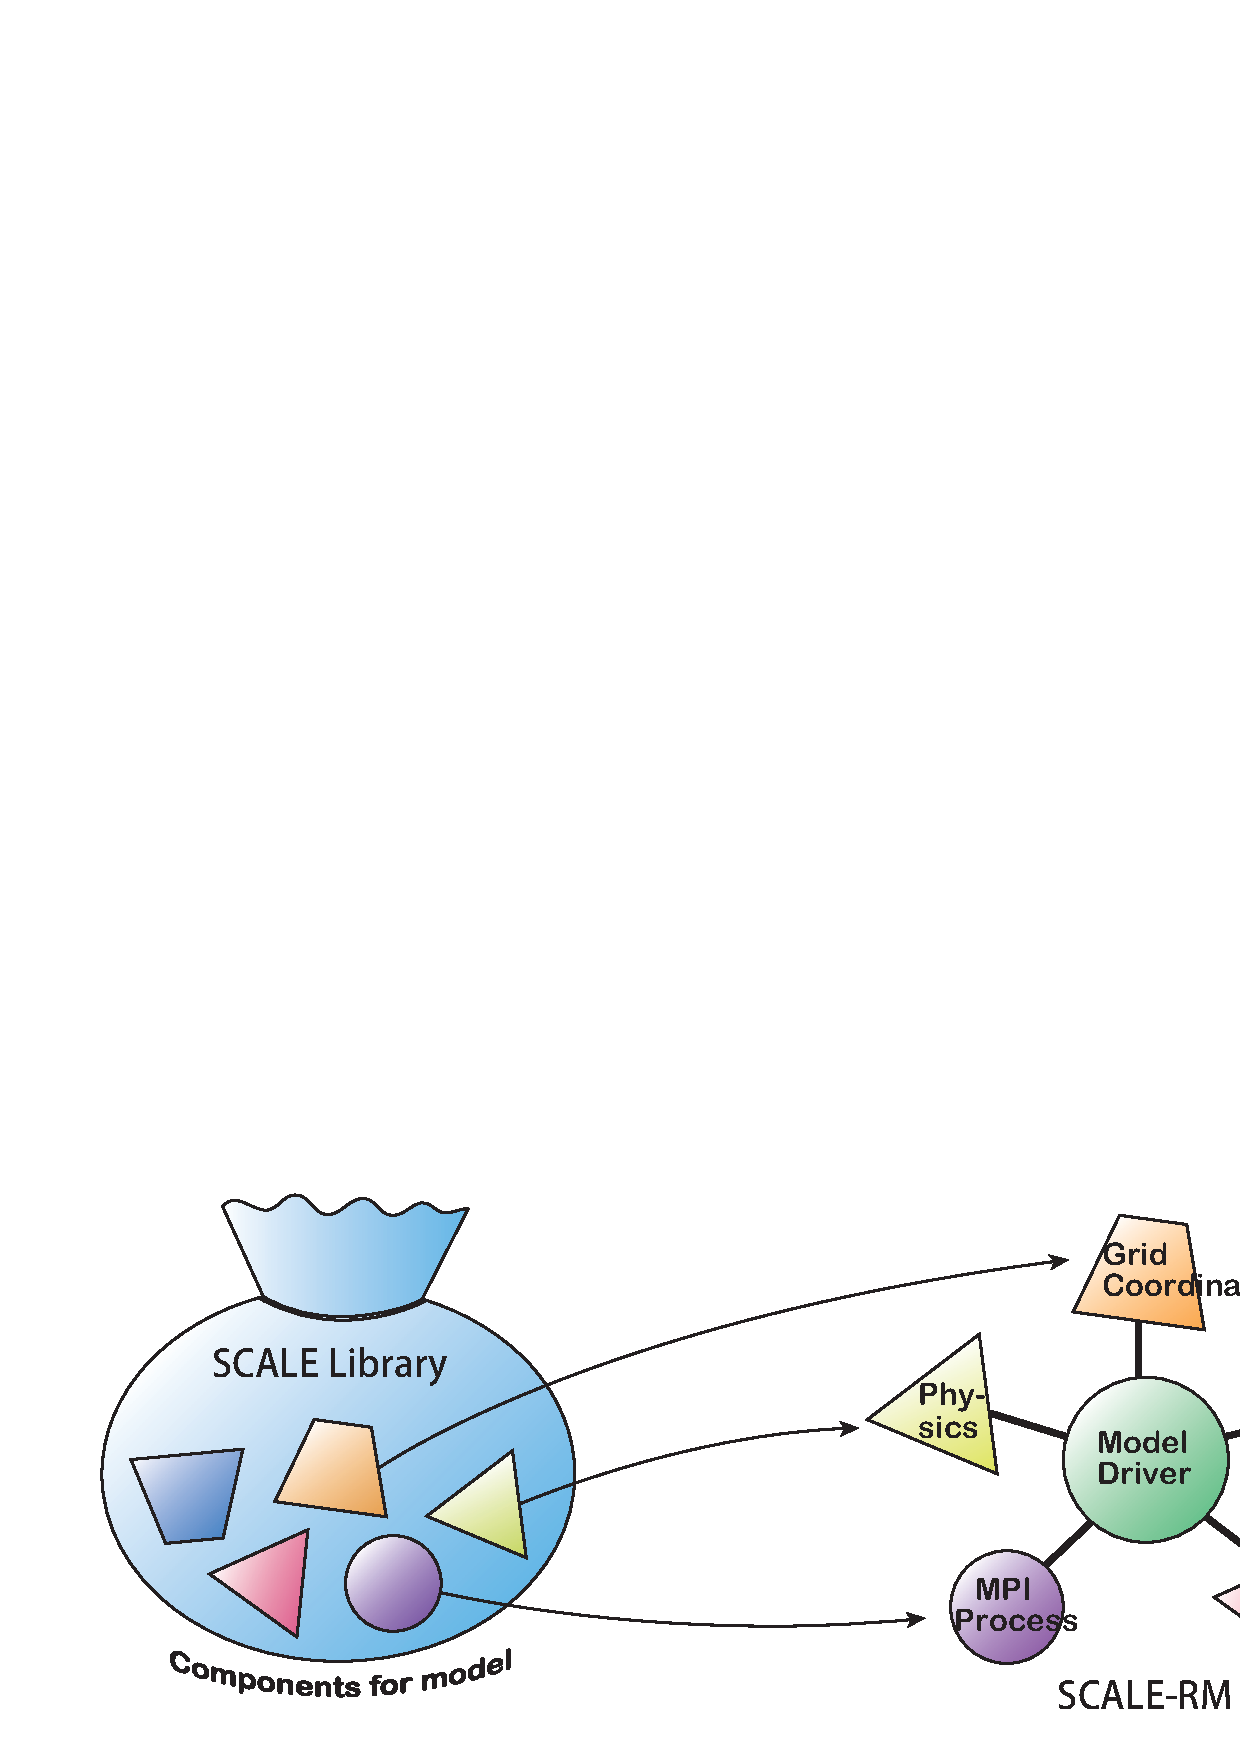
\includegraphics[width=0.9\hsize]{./../../figure/scale.pdf}\\
  \caption{{\scalelib}ライブラリと{\scalerm}(モデル)の関係}
  \label{fig:scale-rm}
\end{center}
\end{figure}



\section{\scalerm の構成}  \label{subsec:sturcture_scale_rm}
%--------------------------------------------------------------%
\scalelib に含まれる全てのコンポーネント中の全てのスキームを、
\scalerm において利用できる。
コンポーネントは3つの部分(フレームワーク、力学コア、物理過程)に分類される。
以下に、\scalerm の現版に実装済みである、様々なスキームを含むコンポーネントを列挙する%
\footnote{
モデルの構成や離散化法の詳細は、
\citet{scale_2015}、\citet{satoy_2015b}、
\citet{nishizawa_2015}を参照されたい。
}。
\\

{\bf フレームワーク}
\begin{itemize}
 \item 実距離に基づいた3次元カーテシアン格子系
 \item MPI通信を用いた2次元領域分割
 \item 各種地図投影法
 \item 領域ネスティングシステム(1 way:親領域$\to$子領域へデータ転送)
   \begin{itemize}
    \item オンライン・ネスティング: 複数ドメインの計算を同時に実行
    \item オフライン・ネスティング:外側ドメインの計算終了後に、その結果を用いて内側ドメインの計算を実行
   \end{itemize}
 \item 複数事例一括実行システム(バルクジョブシステム)
 \item CF 規約\footnote{\url{http://cfconventions.org/}}に基づく \netcdf ファイル I/O
   \begin{itemize}
   \item {\netcdf}3 または {\netcdf}4 形式を選択
   \end{itemize}
 \item 理想実験のための初期値データ生成
 \item 外部データから標高・土地利用区分データを作成
 \item 外部データから初期値・境界値データを作成
   \begin{itemize}
    \item
%      WRF-ARW\footnote{\url{http://www.wrf-model.org/}}、
%      NICAM\footnote{\url{http://nicam.jp/}}、
      \grads \footnote{\url{http://cola.gmu.edu/grads/}}形式での入力に対応
   \end{itemize}
\end{itemize}

{\bf 力学コア}
\begin{itemize}
 \item 支配方程式系: 3次元完全圧縮非静力学方程式系
 \item 空間離散化: 有限体積法
    \begin{itemize}
      \item 2次, 4次, 6次, 8次精度の中心系の移流スキーム
      \item 3次, 5次, 7次精度の風上系の移流スキーム
    \end{itemize}
 \item 時間離散化: 「完全陽解法」(HEVE) または「水平陽解法-鉛直陰解法」(HEVI) から選択
    \begin{itemize}
      \item \citet{Wicker_2002}の3段ルンゲ・クッタスキーム(一般に2次精度)
      \item Heun型の3段ルンゲ・クッタスキーム(3次精度)
      \item 4段のルンゲ・クッタスキーム(4次精度)
      \item 7段のルンゲ・クッタスキーム(6次精度). HEVE でのみ利用可. 
      \item 11段のルンゲ・クッタスキーム(8次精度). HEVE でのみ利用可. 
    \end{itemize}
 \item 非負保証:
    \begin{itemize}
      \item フラックス修正法 \citep[Flux Corrected Transport, FCT; ][]{zalesak_1979}
      \item \citet{Koren_1993}フィルター  (3次精度の風上系の移流スキーム使用時のみ)
    \end{itemize}
 \item 数値フィルタ: 超粘性・拡散 (2, 4, 6, 8 階微分に対応)
 \item 地形: 地形に沿った座標系を用いて表現
\end{itemize}

{\bf 物理過程}
\begin{itemize}
 \item 乱流過程: 以下から選択可能
   \begin{itemize}
    \item \citet{smagorinsky_1963} \& \citet{lilly_1962}型のサブグリッドスケール乱流モデル (\citet{Brown_etal_1994}と\citet{Scotti_1993}による補正)
    \item \citet{Deardorff_1980} サブグリッドスケール乱流モデル
    \item \citet{my_1982,nakanishi_2004}によるlevel 2.5境界層乱流パラメタリゼーション
   \end{itemize}
 \item 雲微物理: 以下から選択可能
   \begin{itemize}
    \item \citet{kessler_1969}による3-class 1モーメントバルクモデル
    \item \citet{tomita_2008}による6-class 1モーメントバルクモデル
    \item \citet{sn_2014}による6-class 2モーメントバルクモデル
    \item \citet{suzuki_etal_2010}によるビン法モデル
   \end{itemize}
 \item 放射過程: \citet{sekiguchi_2008}による相関k分布法ブロードバンド大気放射伝達モデル
 \item 地表面モデル
  \begin{itemize}
   \item 陸面モデル: 熱拡散・バケツモデル
   \item 海洋モデル: 以下から選択可能
   \begin{itemize}
     \item 初期値固定
     \item 外部データ入力
     \item スラブモデル
   \end{itemize}
   \item 都市モデル: \citet{kusaka_2001}による単層キャノピーモデル
   \item バルク交換係数(陸面および海面): 以下から選択可能
   \begin{itemize}
     \item \citet{beljaars_1991,wilson_2001}による普遍関数によるバルク法
     \item \citet{uno_1995}によるLouis 型バルク法
   \end{itemize}
  \end{itemize}
\end{itemize}
